\documentclass{article}

\usepackage[T1]{fontenc} % Umożliwia korzystanie z fontów o kodowaniu T1, które obsługują znaki specjalne używane w językach europejskich.
\usepackage[polish]{babel} % Dostosowuje formatowanie dokumentu do zasad języka polskiego (np. łamanie wierszy, tytuły sekcji).
\usepackage[utf8]{inputenc} % Umożliwia korzystanie z kodowania UTF-8, które obsługuje znaki specjalne i diakrytyczne.
\usepackage{graphicx} % Umożliwia wstawianie obrazów do dokumentu.
\usepackage{subcaption} % Umożliwia tworzenie podpisów dla podobrazów.
\usepackage[margin=2cm]{geometry} % Umożliwia dostosowanie marginesów dokumentu.
\usepackage{listings} % Umożliwia wstawianie kodu źródłowego do dokumentu z odpowiednim formatowaniem.
\usepackage{color} % Umożliwia korzystanie z kolorów w dokumencie.
\usepackage{amsmath} % Rozszerza możliwości formatowania równań matematycznych.
\usepackage{tcolorbox} % Umożliwia tworzenie kolorowych ram dookoła tekstu.
\usepackage{systeme} % Umożliwia tworzenie systemów równań.
\usepackage{indentfirst} % Powoduje, że pierwszy akapit po tytule sekcji jest wcięty.
\usepackage{dsfont} % Umożliwia korzystanie z dodatkowych fontów, np. dla oznaczeń zbiorów liczbowych.
\usepackage{etoolbox} % Pozwala modyfikować pakiety UŻYWAĆ OSTROŻNIE
\usepackage{blindtext} % Pozwala automatycznie pisać blok lorem ipsum
\usepackage{fancyhdr} % Pozwala na stopki u góry i na dole strony
\usepackage{hyperref} % Umożliwia używanie hyperlinków
\hypersetup{
  colorlinks = true,
  linkcolor = black,
  urlcolor = blue,
  pdftitle = {Sprawozdanie z Laboratorium 1} 
}
\patchcmd{\section}{\thispagestyle{plain}}{\thispagestyle{fancy}}{}{}

\definecolor{red}{RGB}{245, 63, 60}
\definecolor{blue}{RGB}{59, 69, 245}
\definecolor{green}{RGB}{59, 245, 117}
\definecolor{yellow}{RGB}{245, 207, 59}

\begin{document}
  \pagestyle{fancy} % pozwala korzystać z pakietu fancyhdr
  \fancyhf{} % clear existing header/footer entries
  \fancyfoot[C]{\thepage}
  \renewcommand{\headrulewidth}{0pt} % Usuń linię na górze strony
  \renewcommand{\footrulewidth}{0.4pt} % Dodaj linię na dole strony  
  \addtolength{\footskip}{0cm} % Zmienia pozycję linii w stopce

  \title{Elektronika Cyfrowa \\ {\large Sprawozdanie z Laboratorium 1}}
  \date{06.03.2024}
  \author{Tomasz Dziób}
  \maketitle

  \tableofcontents
  \pagebreak
  
  \section{Wstęp}
    Poniższe sprawozdanie dotyczy dotyczy pierwszych zajęć których głównym celem było zapoznanie się z obsługą \textit{oscyloskopu} oraz \textit{generatora funkcyjnego}. Zadania skupiają się głównie na przećwiczeniu podstawowych funkcji urządzenia, niezbędnych do zaliczenia następnych laboratoriów.
    \subsection{Użyty Sprzęt}
      \subsubsection{Oscyloskop} 
        Jest to przyrząd elektroniczny służący do obserwowania, obrazowania napięcia w zależności od czasu i badania zależności pomiędzy dwiema wielkościami elektrycznymi, bądź innymi wielkościami fizycznymi reprezentowanymi w postaci elektrycznej.\textsuperscript{[1]}
        \begin{figure}[!ht]
          \begin{center}
              \includegraphics[scale=0.147]{grafiki/2381337-40.jpg}
              \caption{\textit{\href{https://pl.farnell.com/tektronix/mdo3012/oscilloscope-2ch-100mhz-2-5gsps/dp/2381346}{TEKTRONIX MDO3012}} -- dokładny model oscyloskopu używanego  na zajęciach}
          \end{center}
        \end{figure}

      \subsubsection{Generator funkcyjny}
        To urządzenie służące do generowania różnych rodzajów krzywych elektrycznych w szerokim zakresie częstotliwości. Krzywe te moga być cykliczne zlbo jednorazowe, inną funkcją jest też możliwość dodania przesunięcia stałego.

        \begin{figure}[!ht]
          \begin{center}
              \includegraphics[scale=0.075]{grafiki/00291.jpg}
              \caption{\textit{\href{https://www.amazon.in/Skyking-Tektronix-AFG3022B-Arbitrary-Generator/dp/B001JJXG0C}{TEKTRONIX AFG3022B}} -- dokładny model generatora funkcyjnego używanego na zajęciach}
          \end{center}
        \end{figure}

  %\addtolength{\footskip}{-1cm} % Zmienia pozycję linii w stopce
  \fancyfoot[L]{\textsuperscript{[1]}\url{https://pl.wikipedia.org/wiki/Oscyloskop}}
  \fancyfoot[C]{\thepage}
  \pagebreak
  \addtolength{\footskip}{-1cm} % Zmienia pozycję linii w stopce
  \fancyfoot[C]{\quad \\ \thepage}
  \fancyfoot[L]{\textsuperscript{[1][2][3]}\url{http://zefir24.if.uj.edu.pl/pracownia_el/jb_w1.pdf}}

  \subsection{Teoria}
    \subsubsection{Rodzaje sygnałów analogowych}
    Sygnały analogowe to sygnały, które mogą przyjmować dowolną wartość z ciągłego przedziału. Są one ciągłe zarówno w czasie, jak i w amplitudzie. Wyróżniamy kilka rodzajów sygnałów, te z których korzystaliśmy na zajęciach to:
    \begin{itemize}
      \item Sygnał harmoniczny(sinusoidalny)
      \begin{figure}[!ht]
        \begin{center}
            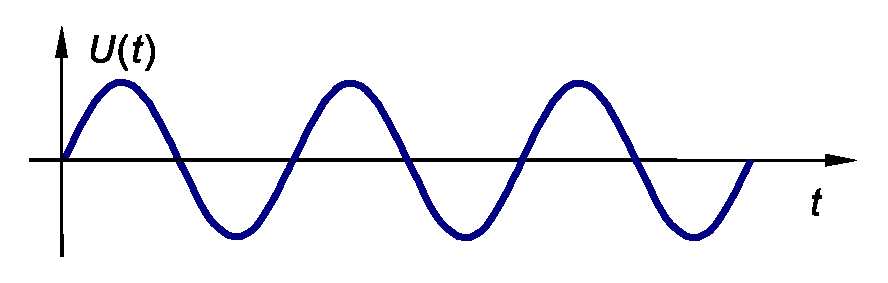
\includegraphics[scale=0.55]{grafiki/syg_har.eps}
            \caption{Zmiana sygnału sinusoidalnego w czasie,\\Źródło:\textsuperscript{[1]}}
        \end{center}
      \end{figure}
      \item Sygnał prostokątny
      \begin{figure}[!ht]
        \begin{center}
            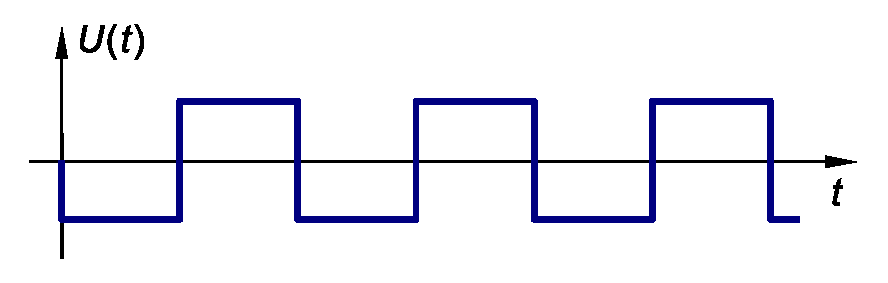
\includegraphics[scale=0.55]{grafiki/syg_pros.eps}
            \caption{Zmiana sygnału sinusoidalnego w czasie,\\Źródło:\textsuperscript{[2]}}
        \end{center}
      \end{figure}
      \item Sygnał trójkątny
      \begin{figure}[!ht]
        \begin{center}
            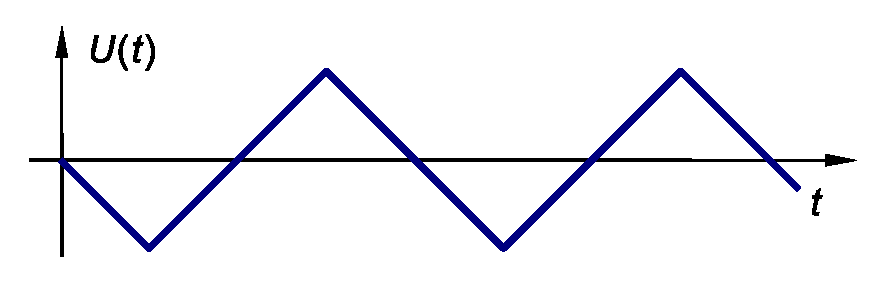
\includegraphics[scale=0.55]{grafiki/syg_troj.eps}
            \caption{Zmiana sygnału sinusoidalnego w czasie,\\Źródło:\textsuperscript{[3]}}
        \end{center}
      \end{figure}
    \end{itemize}

    \subsubsection{Sygnały sinusoidalne}
    Sygnały sinusoidalne są jednym z podstawowych typów sygnałów w analizie sygnałów i systemach. Możemy je zapisać w postaci:
    \begin{equation}
      u(t) = Asin(\omega t + \varphi)
    \end{equation}
    lub
    \begin{equation}
      u(t) = Acos(\omega t + \varphi)
    \end{equation}

    \pagebreak
    \fancyfoot[L]{}

    Podstawowymi parametrami fali sinusoidalnej są:
    \begin{itemize}
      \item $A$ (Amplituda) --- Jest to maksymalna wartość, którą sygnał może osiągnąć. W przypadku sygnału sinusoidalnego, jest to odległość od środka do szczytu (lub dołka) fali.
      \item $f$ (Częstotliwość) ---  określa, ona ile pełnych cykli fali występuje w jednostce czasu. Jej jednostką są herce(Hz).
      \begin{equation}
        f = \frac{\omega}{2\pi}
      \end{equation}
      \item $\varphi$ (Faza) --- opisuje przesunięcie punktu startowego fali sygnału w czasie lub przestrzeni.
      \item $T$ (Okres) --- to czas potrzebny na ukończenie jednego pełnego cyklu fali. \underline{Jest odwrotnością częstotliwości}.
    \end{itemize}

    \begin{figure}[!ht]
      \begin{center}
          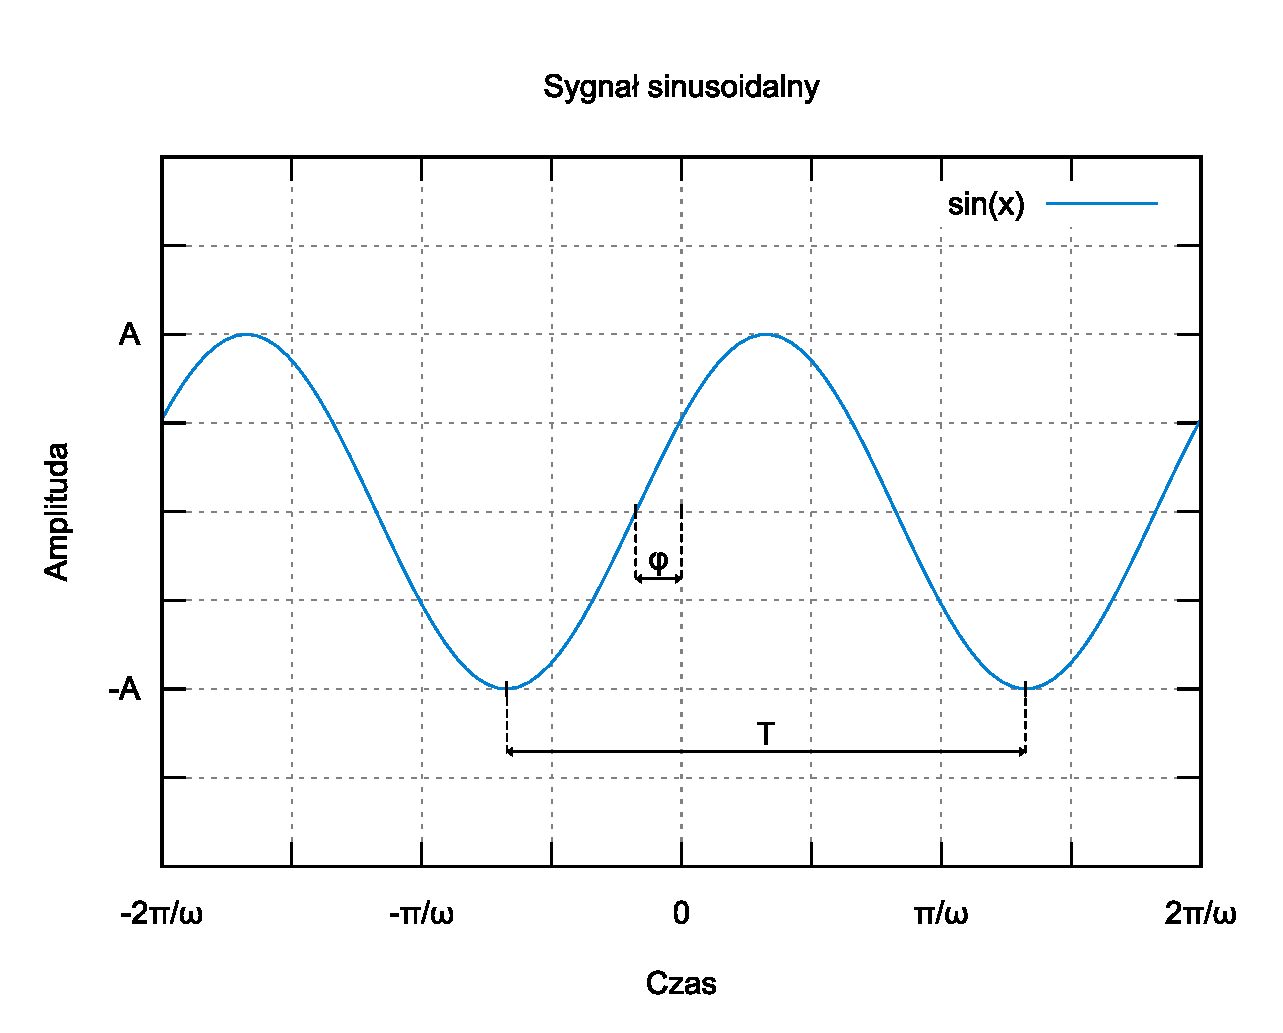
\includegraphics[scale=0.5]{grafiki/sinus.eps}
          \caption{Wizualizacja parametrów na wykresie funkcji sinus,\\Źródło: opracowanie własne}
      \end{center}
    \end{figure}
  
  \section{Ćwiczenia}
    \subsection{Ćwiczenie 1.1}
      Pierwsze zadanie praktyczne polegało na zapoznaniu się z obsługą dwóch sygnałów naraz na oscylatorze. Proste zmiany amplitudy na $500mV$ oraz
      $100mV$. Zadanie zawierało również podstawy ustawania pozycji poszczególnych fal.

      \pagebreak

      W drugiej części zadaniem było podać sygnał wytwarzany przez generator na wejście oscylatora. Dokładnie wyspecyfikowane w poleceniu parametry pozwalały na obeznianie się z podstawowymi funkcjami generatora. Finalnym krokiem było poprawne wyświetlenie uzyskanej fali na oscylatorze. Dzięki wbudowanej w oscylator funkcji ostrzegającej o utracie danych (niepoprawnym wyświetleniu sygnału), jesteśmy wstanie ocenić czy napewno wszystko jest poprawnie ustawione. W przeciwnym razie zostajemy o tym powiadomieni:

      \begin{figure}[!ht]
        \begin{center}
            \includegraphics[scale=0.35]{grafiki/clipping_eg.png}
            \caption{Przykład niepoprawnego wyświetlenia fali,\\Źródło: opracowanie własne}
        \end{center}
      \end{figure}

      Na ekranie pojawia się informacja o utracie danych "{}Clipping pos/neg" w przypadku gdy nie widzimy części pozytywnych oraz negatywnych sygnału. Odpowiednio tylko "{}Clipping positive"{} lub "{}Clipping negative"{} w pozostałych sytuacjach.


      \begin{figure}[!ht]
        \begin{center}
            \includegraphics[scale=0.4]{grafiki/Ramp_freq_15khz_amp_1.55.png}
            \caption{Poprawnie wykonany sygnał trójkątny $A = 1,55 V f = 15 kHz$,\\Źródło: opracowanie własne}
        \end{center}
      \end{figure}

      Trzecią częścią tego zadania było wykonanie porównania metodami \textit{"{}Na oko"{}} z specjalną funkcją wbudowaną w oscylator zwaną \textit{kursorami}. Jest to nic innego jak miarki które możemy dowolnie ustawiać w przestrzeni w celu dokonania pomiarów. 

      \subsubsection{Fala sinusoidalna}
        Sygnał na generatorze posiadał Amplitudę = $1V$ oraz Częstotliwość = $3 kHz$.

        \begin{figure}[!ht]
          \begin{center}
              \includegraphics[scale=0.4]{grafiki/sin_kursory.png}
              \caption{Fala o powyższych parametrach z wyświetlonymi kursorami,\\Źródło: opracowanie własne}
          \end{center}
        \end{figure}

        Uzyskane pomiary przezentują się nastepująco:\\

        \begin{tabular}{|c|c|c|}
          \hline
          & "{}Na oko"{} & Kursory \\
          \hline
          Amplituda & $1V$ & $1,016V$ \\
          \hline
          Częstotliwość & $3,125kHz$ & $3,012kHz$ \\
          \hline
        \end{tabular} \\

        Wyniki "{}Na oko"{} uzyskano wykonując poniższe obliczenia. Aby uzyskać \textbf{Amplitudę} jako jednostkę jednej kratki przyjmujemy ustaloną wcześniej skalę(w tym przypadku $200mV$) oraz mnożymy przez jej rozmiar w kratkach:

        \begin{center}
          ilość kratek $\cdot$ skala Y = Amplituda($V$)
        \end{center}

        \begin{equation}
          5 \cdot 200mV = 1000 mV = 1V
        \end{equation}

        Podobnie sprawa ma się z obliczaniem \textbf{częstotliwości}. Najpierw mnożąc ilość kratek przez przyjętą skalę, uzyskamy okres.

        \begin{center}
          ilość kratek $\cdot$ skala X = Okres($\mu s$)
        \end{center}

        \begin{equation}
          1\frac{3}{5} \cdot 200\mu s = 320 \mu s
        \end{equation}

        \pagebreak

        Ostatnim krokiem jest odwrócenie okresu w celu uzyskania częstotliwości.(Należy pamiętać o zmianie jednostek jeśli chcemy uzyskać wynik w hercach).

        \begin{equation}
          \frac{1}{320 \textcolor{red}{\mu} s} = \frac{1}{320s} \cdot \textcolor{red}{10^6} = 3 125 Hz = 3,125 kHz
        \end{equation}

        Analogiczne obliczenia zostały wykonane dla dwóch pozostałych typów fal.

      \subsubsection{Fala trójkątna}
        Sygnał na generatorze posiadał Amplitudę = $2,5V$, Częstotliwość = $10 kHz$ oraz Fazę = $10^\circ$. Na grafice poniżej zawarta jest również identyczna fala bez fazy, w celu wizualizacji przesunięcia.

        \begin{figure}[!ht]
          \begin{center}
              \includegraphics[scale=0.4]{grafiki/kursor_ver.png}
              \caption{Fala o powyższych parametrach z wyświetlonymi kursorami,\\Źródło: opracowanie własne}
          \end{center}
        \end{figure}

        Uzyskane pomiary:\\

        \begin{tabular}{|c|c|c|}
          \hline
          & "{}Na oko"{} & Kursory \\
          \hline
          Amplituda & $2,5V$ & $2,570V$ \\
          \hline
          Częstotliwość & $10kHz$ & $10kHz$ \\
          \hline
        \end{tabular} \\

        Obliczenia:
        \begin{equation}
          5 \cdot 500mV = 2500 mV = 2.5V
        \end{equation}

        \begin{equation}
          1 \cdot 100\mu s = 100 \mu s
        \end{equation}

        \begin{equation}
          \frac{1}{100 \mu s} = \frac{1}{100s} \cdot 10^6 = 10 000 Hz = 10 kHz
        \end{equation}

      \subsubsection{Fala prostokątna}
        Sygnał na generatorze posiadał Amplitudę = $0,5V$, Częstotliwość = $50 kHz$ oraz Fazę = $180^\circ$. Na grafice poniżej zawarta jest również identyczna fala bez fazy, w celu wizualizacji przesunięcia.

        \begin{figure}[!ht]
          \begin{center}
              \includegraphics[scale=0.4]{grafiki/prost_ver.png}
              \caption{Fala o powyższych parametrach z wyświetlonymi kursorami,\\Źródło: opracowanie własne}
          \end{center}
        \end{figure}

        \pagebreak

        Uzyskane pomiary:\\

        \begin{tabular}{|c|c|c|}
          \hline
          & "{}Na oko"{} & Kursory \\
          \hline
          Amplituda & $0,5V$ & $0,5V$ \\
          \hline
          Częstotliwość & $50kHz$ & $50kHz$ \\
          \hline
        \end{tabular} \\

        Obliczenia:
        \begin{equation}
          5 \cdot 100mV = 500 mV = 0.5V
        \end{equation}

        \begin{equation}
          1 \cdot 20\mu s = 20 \mu s
        \end{equation}

        \begin{equation}
          \frac{1}{20\mu s} = \frac{1}{20s} \cdot 10^6 = 50 000 Hz = 50 kHz
        \end{equation}
        
    \subsection{Ćwiczenie 1.2}
      Polecenie dotyczyło zaobserwowania złożeń dwóch drgań harmonicznych w specjalnym trybie zwanym "X--Y". Drgania te są to tzw. \textit{Krzywe Lissajous}, ich wygląd zależy od amplitudy, częstotliwości i fazy obu sygnałów.

      Cel dydaktyczny tego zadania to tylko i wyłącznie zapoznania się z używanym sprzętem oraz nauka organizacji pracy w pracowni.

      Zostajemy poproszeni o zaprezentowanie 5 uzyskanych kształtów wraz z parametrami:

      \pagebreak

      \subsubsection{Linia}
        \begin{figure}[!ht]
          \begin{center}
              \includegraphics[scale=0.25]{grafiki/linia.png}
              \caption{Kształt linii uzyskany w trybie wyświetlenia "X--Y",\\Źródło: opracowanie własne}
          \end{center}
        \end{figure}
        Wynik uzyskany został za pomocą poniższych parametrów: \\ \\
        Oś X: $A = 1V,f = 3kHz, \varphi = 0^\circ, skala = 500mV$ \\
        Oś Y: $A = 1V,f = 3kHz, \varphi = 0^\circ, skala = 500mV$ \\
        Skala: $40 \mu s$

        \subsubsection{Koło}
        \begin{figure}[!ht]
          \begin{center}
              \includegraphics[scale=0.25]{grafiki/kolo.png}
              \caption{Kształt koła uzyskany w trybie wyświetlenia "X--Y",\\Źródło: opracowanie własne}
          \end{center}
        \end{figure}
        Wynik uzyskany został za pomocą poniższych parametrów: \\ \\
        Oś X: $A = 1V,f = 3kHz, \varphi = 90^\circ, skala = 500mV$ \\
        Oś Y: $A = 1V,f = 3kHz, \varphi = 0^\circ, skala = 500mV$ \\
        Skala: $200 \mu s$

        \pagebreak

        \subsubsection{Elipsa}
        \begin{figure}[!ht]
          \begin{center}
              \includegraphics[scale=0.25]{grafiki/elipsa.png}
              \caption{Kształt elipsy uzyskany w trybie wyświetlenia "X--Y",\\Źródło: opracowanie własne}
          \end{center}
        \end{figure}
        Wynik uzyskany został za pomocą poniższych parametrów: \\ \\
        Oś X: $A = 1V,f = 3kHz, \varphi = 50^\circ, skala = 500mV$ \\
        Oś Y: $A = 1V,f = 3kHz, \varphi = 0^\circ, skala = 500mV$ \\
        Skala: $100 \mu s$

        \subsubsection{Precelek}
        \begin{figure}[!ht]
          \begin{center}
              \includegraphics[scale=0.25]{grafiki/precelek.png}
              \caption{Kształt precelka uzyskany w trybie wyświetlenia "X--Y",\\Źródło: opracowanie własne}
          \end{center}
        \end{figure}
        Wynik uzyskany został za pomocą poniższych parametrów: \\ \\
        Oś X: $A = 2,2V,f = 4kHz, \varphi = 60^\circ, skala = 500mV$ \\
        Oś Y: $A = 2,9V,f = 3kHz, \varphi = 100^\circ, skala = 500mV$ \\
        Skala: $100 \mu s$

        \pagebreak

        \subsubsection{Abstrakcyjny Kształt}
        \begin{figure}[!ht]
          \begin{center}
              \includegraphics[scale=0.25]{grafiki/cos.png}
              \caption{Abstrakcyjny kształt uzyskany w trybie wyświetlenia "X--Y",\\Źródło: opracowanie własne}
          \end{center}
        \end{figure}
        Wynik uzyskany został za pomocą poniższych parametrów: \\ \\
        Oś X: $A = 2V,f = 2kHz, \varphi = 50^\circ, skala = 500mV$ \\
        Oś Y: $A = 2,5V,f = 6kHz, \varphi = 210^\circ, skala = 500mV$ \\
        Skala: $100 \mu s$

    \subsection{Ćwiczenie 1.3}
      Celem ćwiczenia było zaobserwowanie zjawiska dudnień przy użyciu wykorzystując do tego operację \textit{math} z opcją sumy. Zjawisko to zachodzi podczas współbrzmienia dwóch sygnałów o podobnej częstotliwości(w tym przypadku  1,00kHz oraz 1,05kHz)
        \begin{figure}[!ht]
          \begin{center}
              \includegraphics[scale=0.4]{grafiki/dudnienia_kursory.png}
              \caption{Zaobserwowane zjawisko dudnienia,\\Źródło: opracowanie własne}
          \end{center}
        \end{figure}

        Wynik uzyskany został za pomocą kursorów jest następujący:\\ \\
        $\Delta A = 2,950 V$ \\
        $\Delta f = 44,84 Hz$ \\

  \section{Omówienie wyników}
        \subsection{Ćwiczenie 1.1}
          W naszym eksperymencie, porównując wyniki uzyskane obiema metodami, możemy zauważyć, że wartości amplitudy i częstotliwości mierzone za pomocą kursorów oscyloskopu pokrywają się z wartościami rzeczywistymi wyliczonymi ręcznie. Są one obarczone błędem który wynika zapewne z czynnika ludzkiego jakim jest nie dokręcenie pokrętła w idealne miejsce lub lekkiej niestabilności sygnału analogowego.
        \subsection{Ćwiczenie 1.2}
          Podczas wykonywania ćwiczenia uzyskano kilka charakterystycznych kształtów, takich jak linia, koło czy elipsa. Każdy z tych kształtów reprezentuje określone relacje między amplitudami, częstotliwościami i fazami sygnałów wejściowych.
          Na przykład, koło jest wynikiem równych częstotliwości i faz różniących się o 90 stopni, co prowadzi do regularnego, okrągłego kształtu. Natomiast elipsa może być rezultatem nie będących do siebie prostopadłych i różnych od siebie faz, co powoduje rozciągnięcie lub zniekształcenie kształtu.
        \subsection{Ćwiczenie 1.3}
        Zjawisko dudnienia udało się pomyślnie zaobserwować. Jest ono efektem współbrzmienia dwóch sygnałów o zbliżonych częstotliwościach. W przypadku naszego eksperymentu, mieliśmy do czynienia z dwoma sygnałami o częstotliwościach $1,00 kHz$ i $1,05 kHz$.

        Dla zjawisk dudnienia, różnica między częstotliwościami fal (w naszym przypadku $1,05 kHz - 1,00 kHz = 50 Hz$) pokrywa się mniej więcej z wynikem uzyskanym używając kursorów(~$44,84Hz$). Różnica ta wynika niedokładności mojego pomiaru.

        Im większa różnica częstotliwości między falami, tym wyższa jest częstotliwość dudnień.

  \section{Podsumowanie}
    Zapoznanie się z obsługą oscyloskopu oraz generatora funkcyjnego, było kluczowe dla przyszłej pracy w laboratorium na kolejnych zajęciach.

    Korzystając z oscyloskopu, można było obserwować i analizować zmiany napięcia w zależności od czasu oraz badać zależności między różnymi wielkościami elektrycznymi. Natomiast dzięki generatorowi funkcyjnemu była możliwość generowania różnorodnych krzywych elektrycznych w szerokim zakresie częstotliwości oraz eksperymentowania z ich parametrami, takimi jak amplituda, częstotliwość i faza.

    Celem tych laboratoriów było nie tylko zrozumienie teoretycznych podstaw, ale również praktyczne zastosowanie wiedzy. Wykonywanie różnorodnych pomiarów, oraz możliwość eksperymentowania z różnymi parametrami sygnałów, pozwoliła na lepsze zrozumienie ich właściwości i zachowań.
    
    \pagebreak

  \section{Notatki z zeszytu laboratoryjnego}
  \begin{figure}[h]
    \centering
    \begin{minipage}{0.45\textwidth}
        \centering
        \includegraphics[width=0.93\textwidth]{grafiki/notatki1.jpg} 
        \caption{Notatki z zeszytu,\\Źródło: opracowanie własne}
    \end{minipage}\hfill
    \begin{minipage}{0.45\textwidth}
        \centering
        \includegraphics[width=1\textwidth]{grafiki/notatki2.jpg} 
        \caption{Notatki z zeszytu,\\Źródło: opracowanie własne}
    \end{minipage}
\end{figure}

    
\end{document}

